\begin{figure}[htpb]
	\centering\capstart{}
	\subfloat[\(\Re\big\{\pixel{\mathcal{G}}\big\}\)]  % chktex 21
	{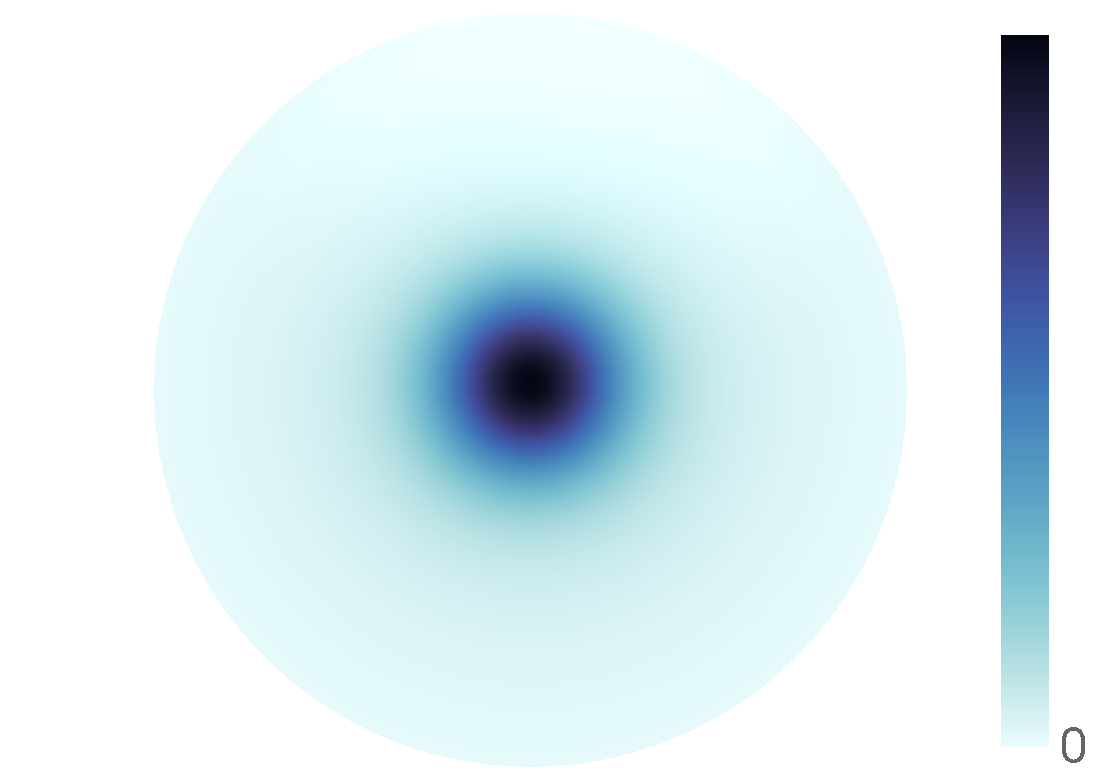
\includegraphics[trim={23 7 3 6},clip,width=.5\textwidth]{gaussian_10sig_L128_res512_real_norm.pdf}}
	\hfill
	\subfloat[\(\Re\big\{\pixel{(\translation{\omega'}\mathcal{G})}\big\}\)]  % chktex 21
	{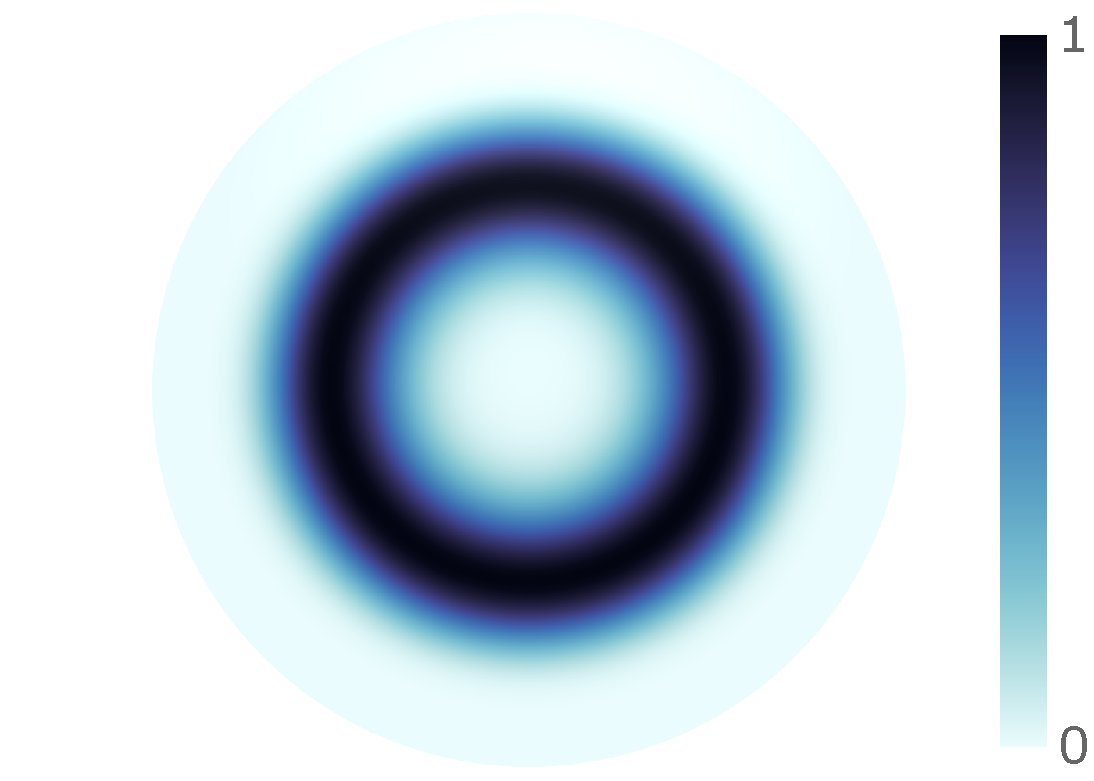
\includegraphics[trim={23 7 3 6},clip,width=.5\textwidth]{gaussian_10sig_L128_translate_alpha3pi4_beta1pi8_res512_real_norm.pdf}}
	\caption[
		A Gaussian on the north pole and then translated
	]{
		Panel (a) presents the standard axisymmetric Gaussian on the north pole (bandlimited at \(L=128\)).
		The Gaussian is then translated to some \(\omega'=(\theta',\phi')\), as shown in panel (b).
		Plainly, the axisymmetric symmetry has been preserved under translation.
		The colour is between zero and one, reflecting the scaled intensity of the field.
	}\label{fig:chapter3_gaussian}
\end{figure}
